\documentclass[a4paper]{report}
\usepackage[14pt]{extsizes}
\usepackage[utf8]{inputenc}
\usepackage[T1]{fontenc}
\usepackage[french]{babel}
\usepackage{makeidx}
\usepackage{graphicx} 
\usepackage{color}

\title{RAPPORT DU PROJET STL \\ TIKZ}
\author{ANCELIN Maxime & DIAKHATE Aminata \\ \\ \\ Encadrant : PESCHANKSI Frédéric}

%\maketable    %pour générer l'index 
\begin{document}
\maketitle


\newpage
\section{Avant propos}
\subsection{Qu'est ce que le logiciel TIKZG?}
\textcolor{red}{TIKZG} est une application permettant la création et la modification de graphes. Il est accessible de tout poste de travail sous Ubuntu.

\subsection{Qu'offre le logiciel TIKZG?}
\begin{itemize}
 \item Il permet d'éditer du code Tikz. L'utilisateur pourra ainsi visualiser le graphe généré.
 \item Il signale à l'utilisateur les éventuels erreurs du code en précisant la ligne concernée.
 \item Il permet à l'utilisateur de modifier graphiquement le résultat d'un code Tikz chargé dans l'application.
 \item Il permet à l'utilisateur d'enregistrer les modifications apportées au code source après modification graphique du graphe.
\end{itemize}
\begin{center}\center{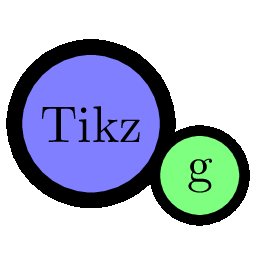
\includegraphics[width=10cm, height=10cm]{img/logo256.png}} \end{center}

\tableofcontents
 \newpage
\section{Installation du logiciel}
\paragraph{Conditions préalables}:
Votre ordinateur doit être équipé du système d'exploitation libre \textcolor{red}{Ubuntu}. Ensuite vous devez à présent récupérer TikzG qui est en logiciel libre.

Après récupération du logiciel, lancez le script d'installation du logiciel "script\_install\_all.sh". Une fois toutes les dépendances installées, ce qui peut prendre près d'une vingtaine de minutes, lancez le logiciel à partir de votre terminal avec la commande "perl tikzg.pl".


\section{Utilisation du logiciel TIKZG}
\subsection{Au démarrage}
Maintenant que vous avez installé votre logiciel, voici la fenêtre que vous devriez avoir au lancement de TIKZG.
\begin{center}\center{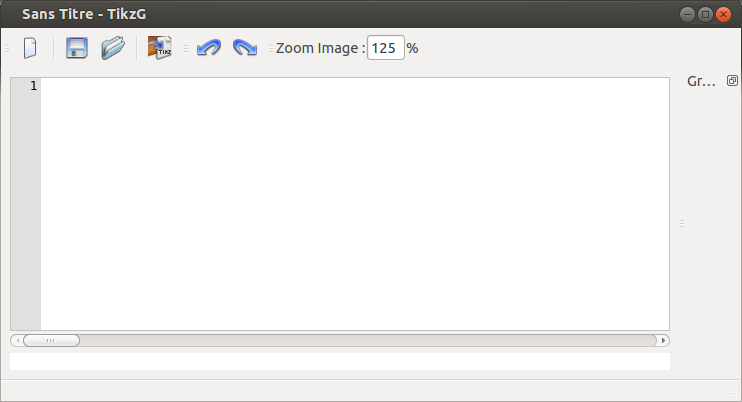
\includegraphics[width=15cm, height=10cm]{img/r_71.png}} \end{center}
\textcolor{red}{Attention}: le design de l'interface peut ne pas être le même, cela dépend de la version de Qt dont vous disposer. Sur l'image ci-dessus la version utilisée est Qt4.

\subsection{Barre de menu}
 \subsubsection{Fichier}
Lorsqu'on clique sur \textcolor{red}{Fichier} dans la barre de menu, on a plusieurs fonctionnalités:
\begin{itemize}
 \item Nouveau(raccourci ctrl+n): permet de créer un fichier vierge dans l'éditeur de texte. 
 \item Ouvrir(raccourci ctrl+o): permet de récupérer un fichier Tikz et de l'ouvrir dans l'éditeur de texte et ainsi pouvoir visualiser le graphe généré.
 \item Enregistrer(raccourci ctrl+s): permet d'enregistrer le code Tikz après lui avoir ajouté une ligne au début "\\begin{tikz}" et une à la fin "\\end{tikz}" afin d'avoir ainsi un code Tikz complet et prêt à être utilisé.
 \item Enregistrer sous(raccourci ctrl+shift+s): même principe que "Enregistrer" et permet en plus de choisir l'emplacement et le nom du fichier.
 \item Exporter: permet d'exporter le graphe obtenu sous forme d'image .png ou de fichier .pdf.
 \item Copier source figure (raccourci ctrl+shift+c): A COMPLETER
 \item Imprimer code tikz: permet comme son intitulé l'indique d'imprimer le code source.
 \item Quitter (raccourci ctrl+q): permet de quitter l'application
\end{itemize}
 \subsubsection{Editer}
Lorsqu'on clique sur \textcolor{red}{Editer} dans la barre de menu, on a plusieurs fonctionnalités:
\begin{itemize}
 \item Défaire(raccourci ctrl+z): permet d'annuler la dernière saisie ajoutée au code. 
 \item Refaire(raccourci ctrl+y): permet de récupérer la dernière saisie annulée.
 \item Couper(raccourci ctrl+x): permet de couper le texte sélectionné.
 \item Copier(raccourci ctrl+c): permet de copier le texte sélectionné.
 \item Coller(raccourci ctrl+v): permet de coller à l'endroit un texte préalablement copié.
 \item Supprimer: permet de supprimer le texte sélectionné.
 \item Tout sélectionner(raccourci ctrl+a): permet de sélectionner tout le code.
\end{itemize}
 \subsubsection{Affichage}
Lorsqu'on clique sur \textcolor{red}{Affichage} dans la barre de menu, on a plusieurs fonctionnalités:
\begin{itemize}
 \item Affichage des numéros de ligne: permet d'afficher ou de cacher les numéros de ligne. 
 \item Coloration syntaxique: permet d'activer ou de désactiver la coloration sytaxique.
 \item Générer image: permet de générer le graphe à partir du code tikz.
\end{itemize}
 \subsubsection{Aide}
Lorsqu'on clique sur \textcolor{red}{Aide} dans la barre de menu on obtient comme seule fonctionnalité l'"A propos" qui nous fournit des renseignements sur l'application.
 \subsubsection{Zoom}
Pour zoomer ou dézoomer le graphe, vous pourrez utiliser la molette de votre souris ou saisir une valeur de zoom dans la barre d'outil.
\subsection{Génération de graphe}
Le graphe est automatiquement généré à partir du code tikz au bout d'une seconde d'inactivité après modication de ce dernier. Voilà un exemple de ce que vous pourrez obtenir avec le code saisi dans l'interface ci-dessous.
\\ \\ \\
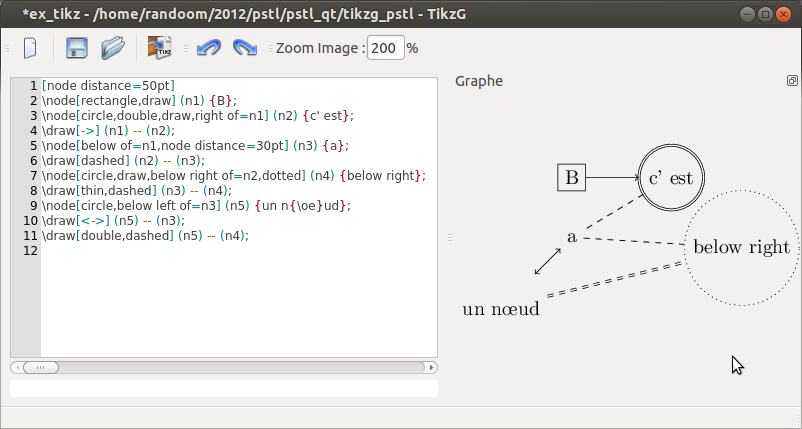
\includegraphics[width=15cm, height=10cm]{img/r_1.png} \\ \\ \\
Et avec un code erroné vous verrez apparaître une fenêtre vous signalant vos erreurs et les lignes concernées comme ceci.
\\
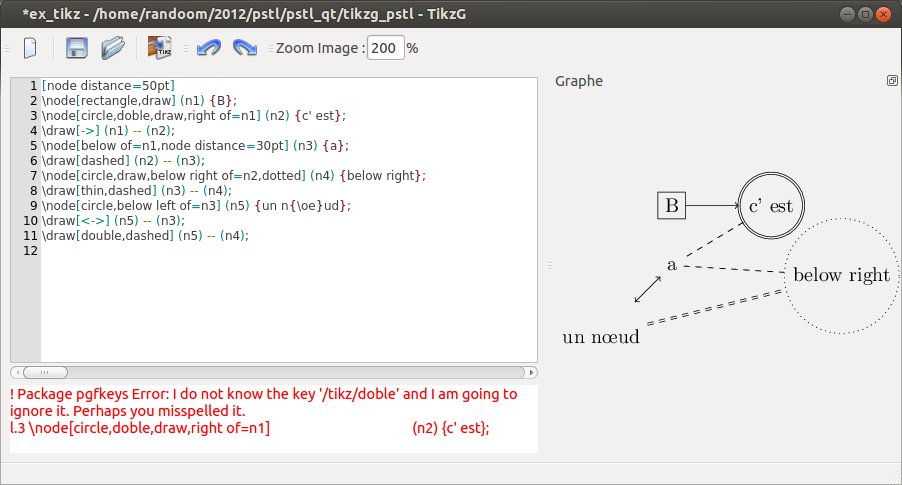
\includegraphics[width=15cm, height=10cm]{img/r_2.png} \\ \\ \\
\subsection{Modification graphique des propriétés d'un n{\oe}ud}
Lorsque vous cliquez sur un n{\oe}ud du graphe, le n{\oe}ud sélectionné se colorie en bleu, ses noeuds relatifs en rose et les arêtes auxquelles il est relié en rouge. Une fenêtre contenant les propriétés du n{\oe}ud en question s'affiche juste en-dessous du graphe. 
Vous devriez alors avoir une interface semblable à l'image ci-dessous.\\ \\ \\
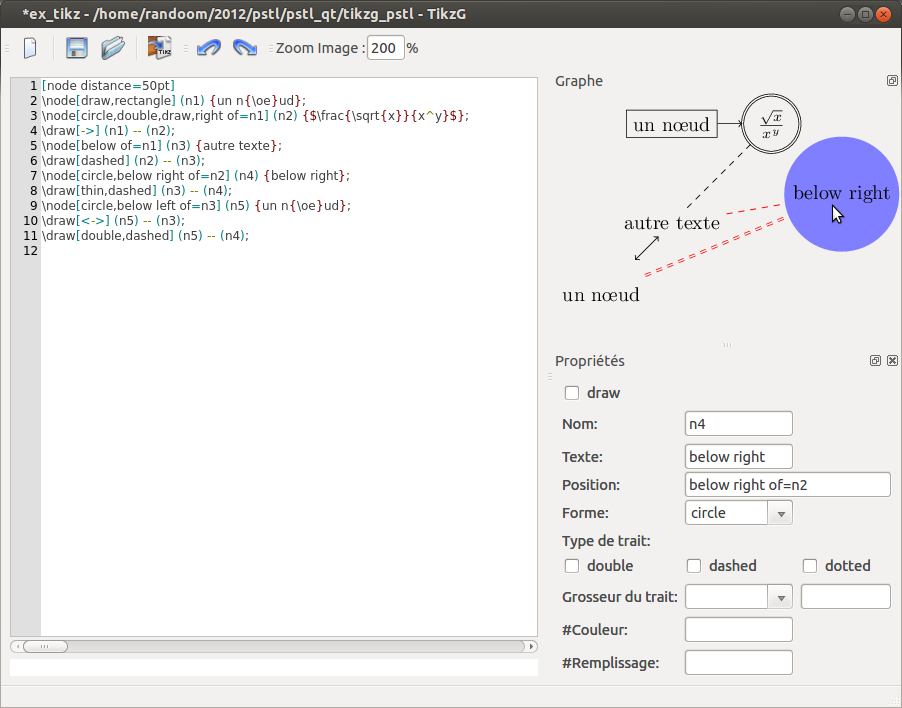
\includegraphics[width=15cm, height=10cm]{img/r_12.png} \\ \\ \\
Vous pourrez grâce à la fenêtre des propriétés choisir de dessiner(resp. cacher) le n{\oe}ud sélectionné en cochant(resp. décochant) la case "draw". Vous pourrez aussi modifier le texte inscrit dans le n{\oe}ud, le nom, la forme ou encore la position du nom en modifiant les champs correspondants dans la fenêtre "Propriétés".
\end{document}

